\section{Variable Time Step Integration}  
%==============================================================================
To enable more efficient simulation of extended term events, variable time step (VTS) integration routines were added to \mbox{PST 4}.
The main assumption behind VTS simulation is that when a system is moving `slowly', larger time steps can accurately capture system dynamics.
Additionally, a viable VTS routine automatically adjusts the time step so that a known error tolerance is always met.
As the time step increases, fewer solutions are required to simulate a set period of time which leads to reductions in the number of calculations and produces a more efficient solution method.
VTS simulations were made possible by using standard MATLAB ODE solvers.
This decision was made to more quickly explore the viability of applying VTS methods to the power system simulation process.

The MATLAB solvers adjust the simulation time step based upon analysis of system derivatives and error tolerances.
To increase efficiency, models that are no longer connected to the system should have their derivatives set to $0$.
Work has been done to zero the derivatives of tripped machines and exciters, but more work can be done to zero derivatives of other attached models (i.e. PSS and governors).

\vspace{3 em}
\noindent \textbf{NOTE:} Variable time step simulation is experimental and should be used with caution!

\pagebreak
%------------------------------ from vts explained
%==============================================================================
\subsection{Solver Control Array (solver\_con)}  
To use VTS integration methods, a user will have to add a \verb|solver_con| to a valid data file.
If a \verb|solver_con| is not specified, Huen's method is used for all time blocks (i.e. default PST 3 behavior).

Between each \verb|sw_con| entry, a \emph{time block} is created that is then solved using a the defined solution method in the \verb|solver_con|.
As such, the \verb|solver_con| array has 1 less row than the \verb|sw_con| array.
An example \verb|solver_con| array is shown in Listing \ref{lst: solverCon ex}.

\begin{lstlisting}[caption={Solver Control Array Example},label={lst: solverCon ex}]
\end{lstlisting}\vspace{-2 em}
\begin{minted}[
		frame=lines,
		framesep=2mm,
		baselinestretch=1.2,
		bgcolor=gray!13,
		fontsize=\footnotesize,
		%linenos,
		breaklines
		]{MATLAB}
%% solver_con format
% A cell with a solver method in each row corresponding to the specified
% 'time blocks' defined in sw_con
%
% Valid solver names:
% huens - Fixed time step default to PST
% ode113 - works well during transients, consistent # of slns, time step stays relatively small
% ode15s - large number of slns during init, time step increases to reasonable size
% ode23 - realtively consistent # of required slns, timstep doesn't get very large
% ode23s - many iterations per step - not efficient...
% ode23t - occasionally hundereds of iterations, most times not... decent performance
% ode23tb - similar to 23t, sometimes more large solution counts

solver_con ={ ...
    'huens'; % pre fault - fault
    'huens'; % fault - post fault 1
    'huens'; % post fault 1 - post fault 2
    'huens'; % post fault 2 - sw_con row 5
    'ode113'; % sw_con row 5 - sw_con row 6 
    'ode23t'; % sw_con row 6  - sw_con row 7  (end)
    };
\end{minted}

\pagebreak
%==============================================================================
\subsection{MATLAB ODE Solvers}
The VTS implementation in PST revolves around using the built in MATLAB ODE solvers.
All these methods perform actions depicted in Figure \ref{fig: MATLAB ode block diagram}.

\begin{figure}[!h]
	\centering
	\footnotesize
	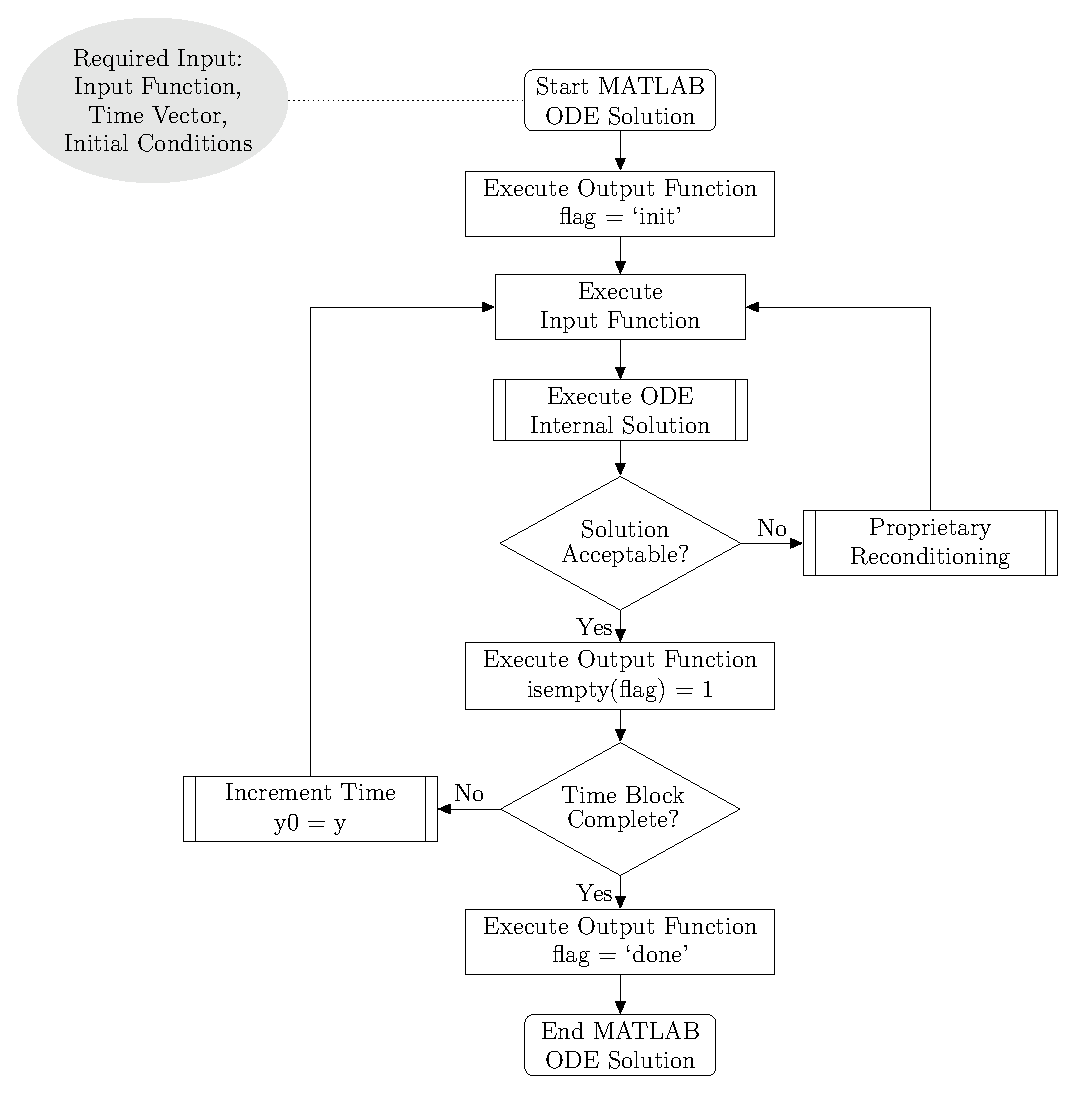
\includegraphics[width=.9\linewidth]{./../../one-offs/200804-ODEblockDiagram/200804-ODEblockDiagram}
	\caption{MATLAB ODE Flow Chart.}
	\label{fig: MATLAB ode block diagram}
\end{figure}%\vspace{-1 em}

\pagebreak
The input to an ODE solver include, an input function, a time interval (time block), initial conditions, and solver options.
The current options used for VTS  that deal with error tolerance levels, initial step size, max step size, and an optional output function are shown in Listing \ref{lst: ode ex}.

\begin{lstlisting}[caption={MATLAB ODE Solver Option Example},label={lst: ode ex}]
\end{lstlisting}\vspace{-2 em}
\begin{minted}[
		frame=lines,
		framesep=2mm,
		baselinestretch=1.2,
		bgcolor=gray!13,
		fontsize=\footnotesize,
	%	linenos,
		breaklines
				]{MATLAB}
% Configure ODE settings
%options = odeset('RelTol',1e-3,'AbsTol',1e-6); % MATLAB default settings
options = odeset('RelTol',1e-4,'AbsTol',1e-7, ...
    'InitialStep', 1/60/4, ...
    'MaxStep',60, ...
    'OutputFcn',outputFcn); % set 'OutputFcn' to function handle
\end{minted}


%==============================================================================
\subsection{Functions Specific to VTS}  
A number of new functions were created to handle data or perform other tasks so that VTS could be integrated into PST.
The following sections provide information about such functions.
% related VTS functions

%==============================================================================
\pagebreak
\subsubsection{vtsInputFcn} 
MATLAB ODE solvers require a passed in function must that returns a vector of derivatives associated with states to integrate.
The \verb|vtsInputFcn| was created to perform this critical task.
The slightly abbreviated input function is shown in Listing \ref{lst: vtsInputFcn}.

\begin{lstlisting}[caption={Abbreviated vtsInputFcn},label={lst: vtsInputFcn}]
\end{lstlisting}\vspace{-2 em}
\begin{minted}[
		frame=lines,
		framesep=2mm,
		baselinestretch=1.2,
		bgcolor=gray!13,
		fontsize=\footnotesize,
	%	linenos,
		breaklines
				]{MATLAB}
function [dxVec] = vtsInputFcn(t, y)
% VTSINPUTFCN passed to ODE solver to perfrom required step operations
%
%   NOTES: Updates and returns g.vts.dxVec
%
%   Input:
%   t - simulation time
%   y - solution vector (initial conditions)
%
%   Output:
%   dxVec - requried derivative vector for ODE solver

global g

handleStDx(g.vts.dataN, y, 2)        % update states at g.vts.dataN with y

initStep(g.vts.dataN)
networkSolutionVTS(g.vts.dataN, t)
dynamicSolution(g.vts.dataN )
dcSolution(g.vts.dataN )

if g.vts.iter == 0
    handleNetworkSln(g.vts.dataN ,1) % save first network solution
end

g.vts.iter = g.vts.iter + 1;         % increment solution iteration counter

handleStDx(g.vts.dataN , [], 1)      % update g.vts.dxVec
dxVec = g.vts.dxVec;                 % return updated derivative vector
end % end vtsInputFcn
\end{minted}

%==============================================================================

\pagebreak
\subsubsection{vtsOutputFcn} 
After each acceptable solution, the ODE solver calls a passed in \emph{output function}.
The \verb|vtsOutputFcn| was created to handle restoring the original network solution, performing the monitor solution, indexing, iteration accumulation, and logging after each step.
The slightly abbreviated VTS output function is shown in Listing \ref{lst: vtsOutputFcn}.

\pagebreak
\begin{lstlisting}[caption={Abbreviated vtsOutputFcn},label={lst: vtsOutputFcn}]
\end{lstlisting}\vspace{-2 em}
\begin{minted}[
		frame=lines,
		framesep=2mm,
		baselinestretch=1.2,
		bgcolor=gray!13,
		fontsize=\footnotesize,
	%	linenos,
		breaklines
				]{MATLAB}
function status = vtsOutputFcn(t,y,flag)
% VTSOUTPUTFCN performs associated flag actions with ODE solvers.
%
%   Input:
%   t - simulation time
%   y - solution vector
%   flag - dictate function action
%
%   Output:
%   status - required for normal operation (return 1 to stop)

global g 
status = 0; % required for normal operation

if isempty(flag)                    % normal step completion
    handleNetworkSln(g.vts.dataN ,2)% restore network to initial solution   
    monitorSolution(g.vts.dataN);   % Perform Line Monitoring and Area Calculations 
    
    if g.sys.livePlotFlag
        livePlot(g.vts.dataN)       % Live plotting
    end
    
    
    g.vts.dataN = g.vts.dataN+1;    % increment logged data index 'dataN'
    g.sys.t(g.vts.dataN) = t;       % log step time
    g.vts.stVec = y;                % update state vector
    handleStDx(g.vts.dataN, y, 2)   % place new solution results into associated globals
    
    g.vts.tot_iter = g.vts.tot_iter + g.vts.iter;   % update total iterations
    g.vts.slns(g.vts.dataN) = g.vts.iter;           % log solution step iterations
    g.vts.iter = 0;                                 % reset iteration counter
    
elseif flag(1) == 'i'               % init solver for new time block
    g.sys.t(g.vts.dataN) = t(1);    % log step time
    handleStDx(g.vts.dataN, y, 2)   % set initial conditions
  
elseif flag(1) == 'd'               % only debug screen output at the moment

end % end if
end % end function
\end{minted}



%==============================================================================
\subsubsection{handleNetworkSln}  
The \verb|handleNetworkSln| function was created to store, and restore, calculated values set to globals during a network solution.
The purpose of this function was to allow for the first network solution performed each step to be carried forward after multiple other network solutions may over-write the calculated values at the same data index.
This over-writing would occur during the MATLAB ODE solver's repeated calls to the input function.
As shown in Listing \ref{lst: handleNetworkSln}, \verb|handlNetworkSln| takes a data index \verb|k| and an operation \verb|flag| as inputs.

\begin{lstlisting}[caption={Function Header for handleNetworkSln},label={lst: handleNetworkSln}]
\end{lstlisting}\vspace{-2 em}
\begin{minted}[
		frame=lines,
		framesep=2mm,
		baselinestretch=1.2,
		bgcolor=gray!13,
		fontsize=\footnotesize,
	%	linenos,
		breaklines
				]{MATLAB}
function handleNetworkSln(k, flag)
% HANDLENETWORKSLN saves or restores the network solution at data index k
%
%   NOTES: Used to reset the newtork values to the initial solution in VTS.
%
%   Input:
%   k - data index to log from and restore to
%   flag - choose funtion operation
%       0 - initialize globals used to store data
%       1 - collect newtork solution values from index k into global vector
%       2 - write stored network solution to globals at index k
\end{minted}

%==============================================================================
\pagebreak
\subsubsection{handleStDx}  
The \verb|handleStDx| function was created to perform the required state and derivative handling to enable the use of internal MATLAB ODE solvers.
Its general operation is probably best described via the internal function documentation shown in Listing \ref{lst: handleStDx}.

\begin{lstlisting}[caption={Function Header for handleStDx},label={lst: handleStDx}]
\end{lstlisting}\vspace{-2 em}
\begin{minted}[
		frame=lines,
		framesep=2mm,
		baselinestretch=1.2,
		bgcolor=gray!13,
		fontsize=\footnotesize,
	%	linenos,
		breaklines
				]{MATLAB}
function handleStDx(k, slnVec, flag)
% HANDLESTDX Performs required state and derivative handling for ODE solvers
%
%   NOTES:  Requires state and derivative values are in the same g.(x) field.
%           Not all flags require same input.
%
%   Input:
%   k - data index
%   flag - choose between operations
%           0 - initialize state and derivative cell array, count states
%           1 - update g.vts.dxVec with col k of derivative fields
%           2 - write slnVec vector of values to associated states at index k
%           3 - update g.vts.stVec with col k of state fields
%   snlVec - Input used to populate states with new values
\end{minted}

The new global structure created in PST 4 enables \verb|handleStDx| to complete the stated operations by relying heavily on dynamic field names. 
Essentially, all required field names, sub-field names, and states are collected into a cell (flag operation 0) that is then iterated through to collect data from, or write data to the appropriate location (all other flag operations).

The usefulness of \verb|handleStDx| is that the standard MATLAB ODE solvers require a single derivative vector as a returned value from some passed in `input function', and each PST model calculates derivatives and places them into various globals. 
Thus, a derivative collection algorithm was needed (flag operation 1).
Once the ODE solver finishes a step, the returned solution vector (of integrated states) must then be parsed into the global state variables associated with the supplied derivatives (flag operation 2).
At the beginning of time blocks that use the MATLAB ODE solvers, an initial conditions vector of all the states related to the derivative vector is a required input (updated via flag operation 3).
To avoid handling function output, global vectors \verb|g.vts.dxVec| and \verb|g.vts.stVec| are used to hold updated derivative and state vector information.

It should be noted that original PST globals follow the same data structure,
however, new models (such as AGC, pwrmod, and ivmmmod) use a slightly different data structure and must be handled in a slightly different way.
As of this writing AGC, pwrmod, and ivmmod functionality has been added to \verb|handleStDx|.
Additional models that require integration may be added to this function as the need arises.





%==========================================================
%\subparagraph{vtsInputFcn and vtsOutputFcn}  
%These functions were described earlier.


\begin{comment}
Document Section 'templates'
%==========================================================
\subparagraph{FcnName}  
FcnDescription
\begin{minted}[
		frame=lines,
		framesep=2mm,
		baselinestretch=1.2,
		bgcolor=gray!13,
		fontsize=\footnotesize,
	%	linenos,
		breaklines
				]{MATLAB}
PasteNewCodeHere
\end{minted}

%==========================================================
\begin{minted}[
		frame=lines,
		framesep=2mm,
		baselinestretch=1.2,
		bgcolor=gray!13,
		fontsize=\footnotesize,
	%	linenos,
		breaklines
				]{MATLAB}
PasteNewCodeHere
\end{minted}
%==========================================================

\end{comment}